

\documentclass{jfds}




\title{How to make a submission to the Journal for Finacial Data Science}
\date{August 18, 2025}
\author{Alicia Vidler}

\begin{document}

\maketitle

\authorbio
      {\textbf{Alicia Vidler} is Post doctoral research fellow at Bar Ilan University, Israel}
  {aliciavidler@gmail.com}
  {Tel Aviv, Israel}
  {(123) 456-789}
\authorbio{\textbf{Copernicus} is Associate Professor of Financial Engineering at Metro State University in Denver, CO}{Copernicus@stars.edu} {123 Finance Rd., Chicago, IL 60601}
  {(312) 555-1234}

\authorbio{\textbf{Einstein} is a researcher at Global Markets Institute in New York, NY}{eintein@someuniversity.org} {123 Finance Rd., Chicago, IL 60601}
  {(312) 555-1234}


\begin{abstract}
In this paper, the author demonstrate how to apply formatting instructions for papers submitted to the Journal of Financial Data Science https://www.pm-research.com/content/iijjfds.
\end{abstract}

\begin{keyfindings}
  \item The authors present a novel method of applying quantum physics to finance.
  \item The computational cost is significantly higher than classical models.
  \item Their model improves precision in volatile market simulations.
\end{keyfindings}

%%leave this here
\newpage


%Put back in the title again

\title{How to make a submission to the Journal for Finacial Data Science}
\printtitleonly


%%Opening intro
This paper opens with an overview of quantum valuation and its applications. Put your opening introduction here.


\title{Quantum Valuation in Modern Finance}
\section{QUANTUM METHODS}

\subsection{Wave Function Modelling}
A few citations to illustrate: \cite{doe2023working}, \cite{smith2021quantum}. And also \cite{morningstar2022data} and \cite{tesler2018market}.

\subsubsection{Pairs trading} 
One example of stat arb that originated from correlations in price movements. Let the variable \(x_1\) be defined.


\begin{figure}[h]
\centering
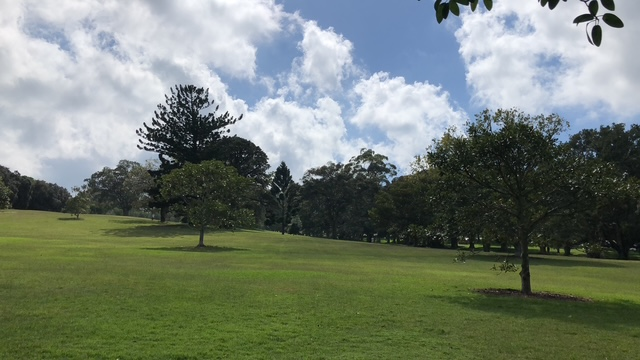
\includegraphics[width=0.6\textwidth]{Tree.JPG}
\caption{Source: Centennial Park by Alicia Vidler '2021}
\end{figure}


\begin{acknowledgments}
The authors thank the reviewers...
\end{acknowledgments}

\newpage

% References should ne on 

\bibliographystyle{JFDS}

\bibliography{references}

\end{document}
